\section{Fremstilling}
\subsection{Projektiler}
Vi udformede projektilerne ved at benytte normale 40mm bordtennisbolde, hvor 3 blev overmalet med akrylmaling for at give dem stærk farve af hhv. rød, grøn og blå. Se Figur \ref{fig:akrylbolde} 
\begin{figure}[H]
	\centering
    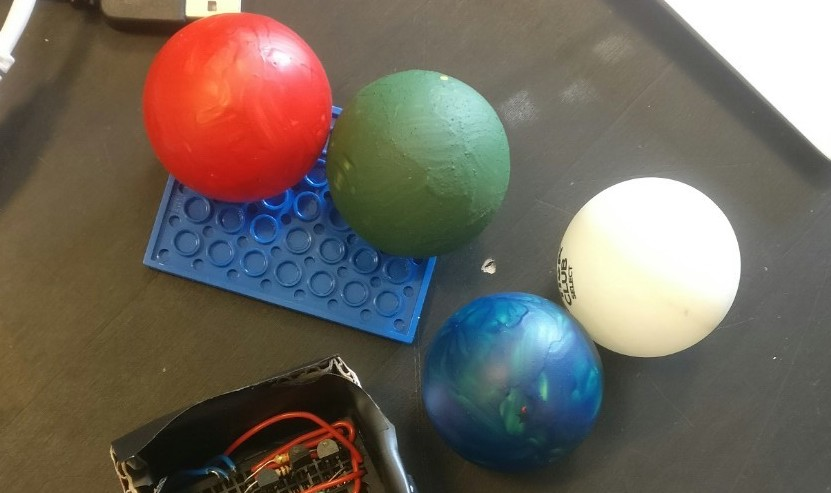
\includegraphics[width=13cm]{figures/2_5fremstilling/akrylbolde.jpeg}
	\caption{Et billede af vores benyttede projektiler}
	\label{fig:akrylbolde}
\end{figure}
\subsection{Fumlebræt-modeller}
Vi lavede en række fumlebrætsmodeller for forskellige dele af det samlede kredsløbet. 
	\begin{figure}[H]
		\centering
	    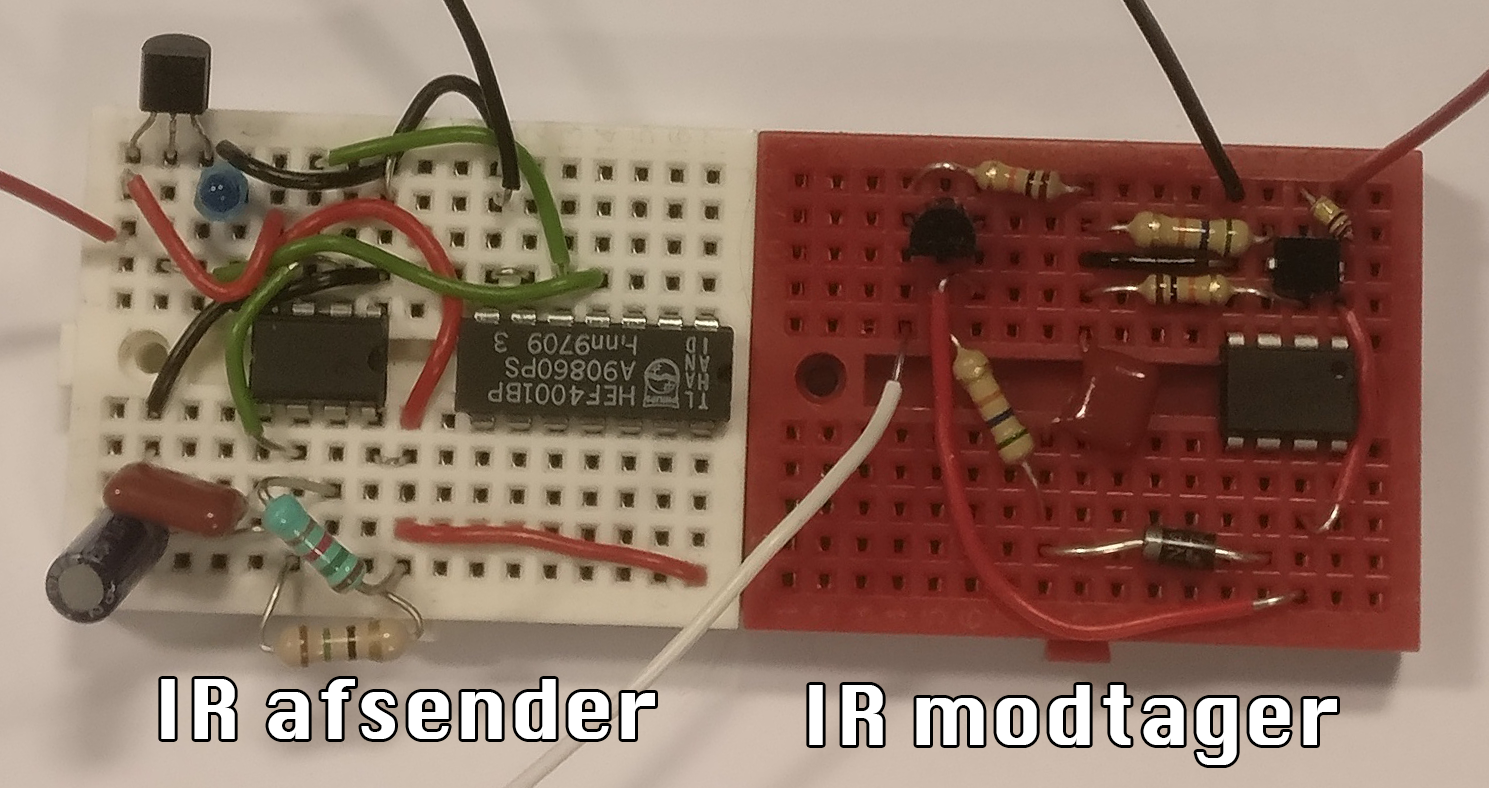
\includegraphics[width=13cm]{figures/2_5fremstilling/prototyper/DanielChrisKreds.png}
		\caption{}
		\label{fig:}
	\end{figure}
\subsection{PCB - fremstilling}\label{subs:pcbfremstilling}
Vi ønskede vores kredsløb på et par mindre PCB. Vi designede to PCB i programmet Livewire i kombination med PCB Wizard. Det ene PCB havde 4 delkredse som skulle skilles fra hinanden ved savning. Disse delkredse var 2 af dem IR-afsender kredsløbet og 2 af dem var IR-modtager kredsløbet. Se det første PCB i Bilag \ref{bilag:afsenderModtagerArtwork}. 

Det andet PCB var et shield til arduinoen der skulle forbindes til diverse kredsløb. Se Bilag \ref{bilag:shieldArtwork}.
\subsubsection{Kemisk fremstilling}
Ved at printe vores print på transfer-papir, kan det benyttes som beskyttelse på kobberplader. Kobberpladerne bliver først UV-belyst, hvor de derefter skylles i en blanding af vand og kaustisk soda indtil printet kan tydeligt ses. Herefter skylles kobberpladen og den lægges i et syrekar indtil de ubeskyttede områder er tilstrækkeligt ætset væk.

\subsubsection{Problemer med printboards}
\todo{Beskriv hvordan PCB-baseret produkt ikke fungrede, har vi nogen mulige forklaringer?} 
% ----------- MULIGE FORKLARINGER
% punkt 1 PCB'et havde muligvist ikke ordenlige forbindelser
% Dette har vi testet ved at bruge et multimeter se om der var gode forbindelser mellem alle punkter på PCB'et
% punkt 2 Der er mulighed for at da PCB'et manglede en ledning eller 2 da det blev lavet på computeren.
% Dette er noget som vi har prøvet at undgå ved at lave så få manuelle ændringer i PCB-wizard så der ikke blev overset nogle forbindelser. 
% punkt 3 Der var komponeter som ikke fungerede ordenligt.
% Det er ikke særlig ofte at komponeter ikke fungere ordenligt når vi bruger dem derfor kan det være at der er en komponent der er blev sat forkert i eller at der er blevet brugt et forkert komponent hvilket også er en del af dette punkt.


\subsection{Endelige prototype}\label{subs:endeligProto}
\begin{figure}[H]
	\centering
    
\includegraphics[width=13cm]{figures/stock.jpg}
	\caption{Billede af endelig produkt}
	\label{fig:endeligPrototype}
\end{figure}




